
%% bare_conf.tex
%% V1.4b
%% 2015/08/26
%% by Michael Shell
%% See:
%% http://www.michaelshell.org/
%% for current contact information.
%%
%% This is a skeleton file demonstrating the use of IEEEtran.cls
%% (requires IEEEtran.cls version 1.8b or later) with an IEEE
%% conference paper.
%%
%% Support sites:
%% http://www.michaelshell.org/tex/ieeetran/
%% http://www.ctan.org/pkg/ieeetran
%% and
%% http://www.ieee.org/

%%*************************************************************************
%% Legal Notice:
%% This code is offered as-is without any warranty either expressed or
%% implied; without even the implied warranty of MERCHANTABILITY or
%% FITNESS FOR A PARTICULAR PURPOSE! 
%% User assumes all risk.
%% In no event shall the IEEE or any contributor to this code be liable for
%% any damages or losses, including, but not limited to, incidental,
%% consequential, or any other damages, resulting from the use or misuse
%% of any information contained here.
%%
%% All comments are the opinions of their respective authors and are not
%% necessarily endorsed by the IEEE.
%%
%% This work is distributed under the LaTeX Project Public License (LPPL)
%% ( http://www.latex-project.org/ ) version 1.3, and may be freely used,
%% distributed and modified. A copy of the LPPL, version 1.3, is included
%% in the base LaTeX documentation of all distributions of LaTeX released
%% 2003/12/01 or later.
%% Retain all contribution notices and credits.
%% ** Modified files should be clearly indicated as such, including  **
%% ** renaming them and changing author support contact information. **
%%*************************************************************************


% *** Authors should verify (and, if needed, correct) their LaTeX system  ***
% *** with the testflow diagnostic prior to trusting their LaTeX platform ***
% *** with production work. The IEEE's font choices and paper sizes can   ***
% *** trigger bugs that do not appear when using other class files.       ***                          ***
% The testflow support page is at:
% http://www.michaelshell.org/tex/testflow/



\documentclass[conference]{IEEEtran}
% Some Computer Society conferences also require the compsoc mode option,
% but others use the standard conference format.
%
% If IEEEtran.cls has not been installed into the LaTeX system files,
% manually specify the path to it like:
% \documentclass[conference]{../sty/IEEEtran}





% Some very useful LaTeX packages include:
% (uncomment the ones you want to load)


% *** MISC UTILITY PACKAGES ***
%
%\usepackage{ifpdf}
% Heiko Oberdiek's ifpdf.sty is very useful if you need conditional
% compilation based on whether the output is pdf or dvi.
% usage:
% \ifpdf
%   % pdf code
% \else
%   % dvi code
% \fi
% The latest version of ifpdf.sty can be obtained from:
% http://www.ctan.org/pkg/ifpdf
% Also, note that IEEEtran.cls V1.7 and later provides a builtin
% \ifCLASSINFOpdf conditional that works the same way.
% When switching from latex to pdflatex and vice-versa, the compiler may
% have to be run twice to clear warning/error messages.






% *** CITATION PACKAGES ***
%
%\usepackage{cite}
% cite.sty was written by Donald Arseneau
% V1.6 and later of IEEEtran pre-defines the format of the cite.sty package
% \cite{} output to follow that of the IEEE. Loading the cite package will
% result in citation numbers being automatically sorted and properly
% "compressed/ranged". e.g., [1], [9], [2], [7], [5], [6] without using
% cite.sty will become [1], [2], [5]--[7], [9] using cite.sty. cite.sty's
% \cite will automatically add leading space, if needed. Use cite.sty's
% noadjust option (cite.sty V3.8 and later) if you want to turn this off
% such as if a citation ever needs to be enclosed in parenthesis.
% cite.sty is already installed on most LaTeX systems. Be sure and use
% version 5.0 (2009-03-20) and later if using hyperref.sty.
% The latest version can be obtained at:
% http://www.ctan.org/pkg/cite
% The documentation is contained in the cite.sty file itself.






% *** GRAPHICS RELATED PACKAGES ***
%
\ifCLASSINFOpdf
  % \usepackage[pdftex]{graphicx}
  % declare the path(s) where your graphic files are
  % \graphicspath{{../pdf/}{../jpeg/}}
  % and their extensions so you won't have to specify these with
  % every instance of \includegraphics
  % \DeclareGraphicsExtensions{.pdf,.jpeg,.png}
\else
  % or other class option (dvipsone, dvipdf, if not using dvips). graphicx
  % will default to the driver specified in the system graphics.cfg if no
  % driver is specified.
  % \usepackage[dvips]{graphicx}
  % declare the path(s) where your graphic files are
  % \graphicspath{{../eps/}}
  % and their extensions so you won't have to specify these with
  % every instance of \includegraphics
  % \DeclareGraphicsExtensions{.eps}
\fi
% graphicx was written by David Carlisle and Sebastian Rahtz. It is
% required if you want graphics, photos, etc. graphicx.sty is already
% installed on most LaTeX systems. The latest version and documentation
% can be obtained at: 
% http://www.ctan.org/pkg/graphicx
% Another good source of documentation is "Using Imported Graphics in
% LaTeX2e" by Keith Reckdahl which can be found at:
% http://www.ctan.org/pkg/epslatex
%
% latex, and pdflatex in dvi mode, support graphics in encapsulated
% postscript (.eps) format. pdflatex in pdf mode supports graphics
% in .pdf, .jpeg, .png and .mps (metapost) formats. Users should ensure
% that all non-photo figures use a vector format (.eps, .pdf, .mps) and
% not a bitmapped formats (.jpeg, .png). The IEEE frowns on bitmapped formats
% which can result in "jaggedy"/blurry rendering of lines and letters as
% well as large increases in file sizes.
%
% You can find documentation about the pdfTeX application at:
% http://www.tug.org/applications/pdftex





% *** MATH PACKAGES ***
%
%\usepackage{amsmath}
% A popular package from the American Mathematical Society that provides
% many useful and powerful commands for dealing with mathematics.
%
% Note that the amsmath package sets \interdisplaylinepenalty to 10000
% thus preventing page breaks from occurring within multiline equations. Use:
%\interdisplaylinepenalty=2500
% after loading amsmath to restore such page breaks as IEEEtran.cls normally
% does. amsmath.sty is already installed on most LaTeX systems. The latest
% version and documentation can be obtained at:
% http://www.ctan.org/pkg/amsmath





% *** SPECIALIZED LIST PACKAGES ***
%
%\usepackage{algorithmic}
% algorithmic.sty was written by Peter Williams and Rogerio Brito.
% This package provides an algorithmic environment fo describing algorithms.
% You can use the algorithmic environment in-text or within a figure
% environment to provide for a floating algorithm. Do NOT use the algorithm
% floating environment provided by algorithm.sty (by the same authors) or
% algorithm2e.sty (by Christophe Fiorio) as the IEEE does not use dedicated
% algorithm float types and packages that provide these will not provide
% correct IEEE style captions. The latest version and documentation of
% algorithmic.sty can be obtained at:
% http://www.ctan.org/pkg/algorithms
% Also of interest may be the (relatively newer and more customizable)
% algorithmicx.sty package by Szasz Janos:
% http://www.ctan.org/pkg/algorithmicx




% *** ALIGNMENT PACKAGES ***
%
%\usepackage{array}
% Frank Mittelbach's and David Carlisle's array.sty patches and improves
% the standard LaTeX2e array and tabular environments to provide better
% appearance and additional user controls. As the default LaTeX2e table
% generation code is lacking to the point of almost being broken with
% respect to the quality of the end results, all users are strongly
% advised to use an enhanced (at the very least that provided by array.sty)
% set of table tools. array.sty is already installed on most systems. The
% latest version and documentation can be obtained at:
% http://www.ctan.org/pkg/array


% IEEEtran contains the IEEEeqnarray family of commands that can be used to
% generate multiline equations as well as matrices, tables, etc., of high
% quality.




% *** SUBFIGURE PACKAGES ***
%\ifCLASSOPTIONcompsoc
%  \usepackage[caption=false,font=normalsize,labelfont=sf,textfont=sf]{subfig}
%\else
%  \usepackage[caption=false,font=footnotesize]{subfig}
%\fi
% subfig.sty, written by Steven Douglas Cochran, is the modern replacement
% for subfigure.sty, the latter of which is no longer maintained and is
% incompatible with some LaTeX packages including fixltx2e. However,
% subfig.sty requires and automatically loads Axel Sommerfeldt's caption.sty
% which will override IEEEtran.cls' handling of captions and this will result
% in non-IEEE style figure/table captions. To prevent this problem, be sure
% and invoke subfig.sty's "caption=false" package option (available since
% subfig.sty version 1.3, 2005/06/28) as this is will preserve IEEEtran.cls
% handling of captions.
% Note that the Computer Society format requires a larger sans serif font
% than the serif footnote size font used in traditional IEEE formatting
% and thus the need to invoke different subfig.sty package options depending
% on whether compsoc mode has been enabled.
%
% The latest version and documentation of subfig.sty can be obtained at:
% http://www.ctan.org/pkg/subfig




% *** FLOAT PACKAGES ***
%
%\usepackage{fixltx2e}
% fixltx2e, the successor to the earlier fix2col.sty, was written by
% Frank Mittelbach and David Carlisle. This package corrects a few problems
% in the LaTeX2e kernel, the most notable of which is that in current
% LaTeX2e releases, the ordering of single and double column floats is not
% guaranteed to be preserved. Thus, an unpatched LaTeX2e can allow a
% single column figure to be placed prior to an earlier double column
% figure.
% Be aware that LaTeX2e kernels dated 2015 and later have fixltx2e.sty's
% corrections already built into the system in which case a warning will
% be issued if an attempt is made to load fixltx2e.sty as it is no longer
% needed.
% The latest version and documentation can be found at:
% http://www.ctan.org/pkg/fixltx2e


%\usepackage{stfloats}
% stfloats.sty was written by Sigitas Tolusis. This package gives LaTeX2e
% the ability to do double column floats at the bottom of the page as well
% as the top. (e.g., "\begin{figure*}[!b]" is not normally possible in
% LaTeX2e). It also provides a command:
%\fnbelowfloat
% to enable the placement of footnotes below bottom floats (the standard
% LaTeX2e kernel puts them above bottom floats). This is an invasive package
% which rewrites many portions of the LaTeX2e float routines. It may not work
% with other packages that modify the LaTeX2e float routines. The latest
% version and documentation can be obtained at:
% http://www.ctan.org/pkg/stfloats
% Do not use the stfloats baselinefloat ability as the IEEE does not allow
% \baselineskip to stretch. Authors submitting work to the IEEE should note
% that the IEEE rarely uses double column equations and that authors should try
% to avoid such use. Do not be tempted to use the cuted.sty or midfloat.sty
% packages (also by Sigitas Tolusis) as the IEEE does not format its papers in
% such ways.
% Do not attempt to use stfloats with fixltx2e as they are incompatible.
% Instead, use Morten Hogholm'a dblfloatfix which combines the features
% of both fixltx2e and stfloats:
%
% \usepackage{dblfloatfix}
% The latest version can be found at:
% http://www.ctan.org/pkg/dblfloatfix




% *** PDF, URL AND HYPERLINK PACKAGES ***
%
%\usepackage{url}
% url.sty was written by Donald Arseneau. It provides better support for
% handling and breaking URLs. url.sty is already installed on most LaTeX
% systems. The latest version and documentation can be obtained at:
% http://www.ctan.org/pkg/url
% Basically, \url{my_url_here}.




% *** Do not adjust lengths that control margins, column widths, etc. ***
% *** Do not use packages that alter fonts (such as pslatex).         ***
% There should be no need to do such things with IEEEtran.cls V1.6 and later.
% (Unless specifically asked to do so by the journal or conference you plan
% to submit to, of course. )


% correct bad hyphenation here
\hyphenation{op-tical net-works semi-conduc-tor}

\usepackage[utf8]{inputenc}
\usepackage{ae}
\usepackage{multirow}

\usepackage{amsmath}
% --------------------------------------------------

\usepackage{graphicx}
\usepackage{float}

\usepackage[lined,ruled,boxed]{algorithm2e}
%\usepackage{algorithmic}


\usepackage{epstopdf}
\usepackage[table]{xcolor}
\usepackage{booktabs}

\usepackage{caption}
\usepackage{subcaption}
%\usepackage{hyperlinks}
\usepackage{url}

%\usepackage{amsrefs}


%-----------------------
\usepackage{mathtools, nccmath}
\newcommand{\N}{\mathbb N}
\newcommand{\Q}{\mathbb Q}
\newcommand{\R}{\mathbb R}

\usepackage{xparse}

\DeclarePairedDelimiterX{\set}[1]{\{}{\}}{\setargs{#1}}
\NewDocumentCommand{\setargs}{>{\SplitArgument{1}{;}}m}
{\setargsaux#1}
\NewDocumentCommand{\setargsaux}{mm}
{\IfNoValueTF{#2}{#1} {#1\,\delimsize|\,\mathopen{}#2}}%{#1\:;\:#2}

\parindent = 0pt
%\renewcommand{\baselinestretch}{0.99}
%\setlength{\belowcaptionskip}{-6 pt}
\usepackage{amsfonts}
\newcommand{\commentib}[1]{{\color{blue} [IB: #1]}}

\newtheorem{myDefinition}{Definition}

\begin{document}

\title{Radio Communication to Control and Run an Autonomous Mission for UAVs via a Mobile App}


\author{\IEEEauthorblockN{Thiago R. F. Cavalcante}
\IEEEauthorblockA{Electronic and Information\\Research Center\\
Federal University of Amazonas\\
Amazonas, Manaus\\
Email: thiagorodrigoengcomp@gmail.com}
\and
\IEEEauthorblockN{Erickson H. da S. Alves}
\IEEEauthorblockA{Electronic and Information\\Research Center\\
Federal University of Amazonas\\
Amazonas, Manaus\\
Email: erickson.higor@gmail.com}
\and
\IEEEauthorblockN{Celso B. Carvalho}
\IEEEauthorblockA{Electronic and Information\\Research Center\\
Federal University of Amazonas\\
Amazonas, Manaus\\
Email: celsocarvalho75@gmail.com}}

% conference papers do not typically use \thanks and this command
% is locked out in conference mode. If really needed, such as for
% the acknowledgment of grants, issue a \IEEEoverridecommandlockouts
% after \documentclass

% for over three affiliations, or if they all won't fit within the width
% of the page, use this alternative format:
% 
%\author{\IEEEauthorblockN{Michael Shell\IEEEauthorrefmark{1},
%Homer Simpson\IEEEauthorrefmark{2},
%James Kirk\IEEEauthorrefmark{3}, 
%Montgomery Scott\IEEEauthorrefmark{3} and
%Eldon Tyrell\IEEEauthorrefmark{4}}
%\IEEEauthorblockA{\IEEEauthorrefmark{1}School of Electrical and Computer Engineering\\
%Georgia Institute of Technology,
%Atlanta, Georgia 30332--0250\\ Email: see http://www.michaelshell.org/contact.html}
%\IEEEauthorblockA{\IEEEauthorrefmark{2}Twentieth Century Fox, Springfield, USA\\
%Email: homer@thesimpsons.com}
%\IEEEauthorblockA{\IEEEauthorrefmark{3}Starfleet Academy, San Francisco, California 96678-2391\\
%Telephone: (800) 555--1212, Fax: (888) 555--1212}
%\IEEEauthorblockA{\IEEEauthorrefmark{4}Tyrell Inc., 123 Replicant Street, Los Angeles, California 90210--4321}}




% use for special paper notices
%\IEEEspecialpapernotice{(Invited Paper)}




% make the title area
\maketitle

% As a general rule, do not put math, special symbols or citations
% in the abstract
\begin{abstract}
This paper presents the development of a methodology to carry out missions in a production line environment using an unmanned aerial vehicle (UAV). The used UAV is equipped with a robotic gripper, which consists in an industrial scenario with an input warehouse, production lines, and a product depot. The mission, \textit{i.e.}, the production of a product, executed by the drone is previously planned, optimizing the traveled distance. We have implemented our methodology in an Android application, which uses radio waves to communicate with the UAV, sending commands and receiving statuses. It is presented how the mobile application is useful to assist in the supervisioning process for line managers/leaders.
\end{abstract}

% no keywords




% For peer review papers, you can put extra information on the cover
% page as needed:
% \ifCLASSOPTIONpeerreview
% \begin{center} \bfseries EDICS Category: 3-BBND \end{center}
% \fi
%
% For peerreview papers, this IEEEtran command inserts a page break and
% creates the second title. It will be ignored for other modes.
\IEEEpeerreviewmaketitle



\section{Introduction}
% no \IEEEPARstart
\label{sec:introduction}

Logistics has become a competitive and fundamental factor for organizations, involving the management, conservation, and supervision of freight transport. In addition, excellent logistics means customer satisfaction; so speed is still an important factor in a successful logistics process~\cite{drone4logistic}. Currently, one of the solutions to this type of problem is the use of unmanned aerial vehicles (UAVs). Nowadays, UAVs are mostly remotely piloted vehicles (RPV), since their operations are carried out by ground operators. If the tasks performed by a UAV are performed autonomously, it would relieve the work of these operators, since they perform tedious and repetitive tasks~\cite{pascarella2013autonomic}.

One possible improvement of these logistics systems is the increase of the UAVs automation, which results in costs minimization. Consequently, investments and studies related to stand-alone UAVs are important to the smart factories development~\cite{hern2014dhl}. However, one of the main problems for using autonomous UAVs is the system's reliability and intelligence. Thus, increased employment of autonomous UAVs requires the development of devices, which are able to perform tasks and interact with the environment in an intelligent and reliable way.

Autonomous UAVs need to know what will happen in a future instant and what is the best decision to make at the present time; therefore, they require strategies not only to decompose their missions into meaningful sub-tasks, but also to track progress toward mission goals and the evolution of these tasks relative to the autonomous UAVs capabilities~\cite{finn2012developments}. As a consequence, in order to successfully perform a mission, it is recommended to perform task planning~\cite{finn2012developments}. Mission planning problems consist of planning events to meet certain requirements and objectives~\cite{krozel1988search}. Therefore, planning events is one of the main challenges faced in solving this problem.

Both academy and industry have been researching about evaluation and optimization of mission planning in the last years. In \cite{schwarz2012towards} is used ant colony to optimize UAV missions. Another paper investigates energy consumption for a factory and evaluates the logistic planning processes using statistical metrics of evaluation~\cite{muller2012analyzing}.

In this work we present a methodology to carry out a mission, \textit{i.e.}, a client order, in a production environment. Such mission is previously planned, so that the distance traveled by the UAV is optimized. Moreover, these components are implemented in an Android application, which uses radio waves to communicate with the drone. The mobile app is useful for leaders and/or managers, since they are able to supervise production lines in real-time, checking statuses and acting on failures.

In summary, the main contributions of this study are:
\begin{itemize}
\item an Android app to supervise production lines;
\item methods to control and communicate with the drone using a smartphone;
\item a mission planner to carry out client orders, prioritizing the distance traveled by the UAV.
\end{itemize}
	
\textit{Outline}. Section~\ref{sec:background} provides the fundamentals of mission planning and optimization problems. Section~\ref{sec:uav} describes the UAV movement system used in this work. Section~\ref{sec:method} explains the proposed evaluation methodology in further details. Section~\ref{sec:results} describes the experimental procedures and results in order to explore and demonstrate the potential of methodology, and, finally, Section~\ref{sec:conclusao} concludes this study and describes future work.

%--------------------------------------------
\section{Preliminaries}
\label{sec:background}
%--------------------------------------------

%--------------------------------------------
\subsection{Terminology}
\label{sec:terms}
%--------------------------------------------

Key definitions related to the case study and the application developed in this study need to be clarified. All definitions below are adopted in the remainder of this study.

\begin{myDefinition} 
\textbf{(Mission Command)} 
Mission Command is a command created to execute a task such as to go from one location to another, get a package using a robot gripper, and land a UAV.
\label{def:missioncommand}
\end{myDefinition}

\begin{myDefinition}
\textbf{(Mission)} 
Mission is the set of steps and mission commands that accomplish the clients order.
\label{def:mission}
\end{myDefinition}

\begin{myDefinition}
\textbf{(Warehouse)}
Warehouse is the set of stored raw material available until the moment of entering the productive process. The raw materials, \textit{i.e.}, the inputs available in this work are inputs A, B, and C.
\label{def:almoxarifado}
\end{myDefinition}

\begin{myDefinition} 
\textbf{(Order)}
Order is the requisition of products made by the client. In this study, the products are of type X and Y.
\label{def:pedido}
\end{myDefinition}

\begin{myDefinition}
\textbf{(Production Time)}
Production time is the time required to produce a product X or Y, after making available all the needed inputs for the production, given by the production rule.
\label{def:tempoProducao}
\end{myDefinition}

\begin{myDefinition}
 \textbf{(Production Rule)}
Production rule describes what and how many inputs are needed to produce a particular product.
\label{def:regraProducao}
\end{myDefinition}

\begin{myDefinition}
\textbf{(Mission Planner)}
Mission planner is the agent who performs the planning of a mission, that is, produce all steps and commands needed to carry out a given mission.
\label{def:planejadorMissao}
\end{myDefinition}

\begin{myDefinition}
 \textbf{(Mission File)}
The mission file is a file that is created for the context of this work, with the extension \textsc{.mission} containing the mission itself.
\label{def:arquivoMissao}
\end{myDefinition}

\begin{myDefinition}
 \textbf{(Movement Function)}
The movement function are functions created in Python using the drokekit API to send commands to the UAV by MAVLink protocol.
\label{def:movFunc}
\end{myDefinition}

\begin{myDefinition}
 \textbf{(Production Mission)}
The production mission is the set of steps to produce all the product required by the client.
\label{def:prodMission}
\end{myDefinition}


%--------------------------------------------
%\subsection{DroneKit-Android’s API}
%\label{subsec:dronekit}
%--------------------------------------------

%--------------------------------------------
\subsection{UAV Iris+}
\label{subsec:uaviris}
%--------------------------------------------

The Iris+, introduced by 3DRobotics in Fall 2014, is a 550mm class (measured motor-to-motor) ready-to-fly quadcopter \cite{iris+}. It is powered by a 5100mAh battery driving 4 950kV motors through a 4-in-1 electronic speed controller. It includes a Pixhawk flight control board (described below), an internal uBlox GPS with integrated 3-axis compass for navigation, and a 915MHz radio (or 433MHz, depending on country) for communication with a ground control station. Also included is a full-featured remote control transmitter with a preconfigured receiver onboard the drone. The Iris+ has an advertised flight time of 16-22 min. As of January 2016, the Iris+ retails for \$600, very reasonable for a vehicle with its capabilities.

	\begin{figure}[H]
	\centering
	\includegraphics[width=1.0\columnwidth]{iris.eps}
	\caption{The 3DR Iris+.\label{fig:iris}}
	\end{figure}

Control of the Iris+ is facilitated via the Pixhawk flight control board \cite{meier2011pixhawk}. Developed by researchers at ETH Zurich, the Pixhawk is open source and very widely adopted. It is suitable for use in copters, planes and ground-based rovers. Connectivity options are numerous, allowing for use of a wide array of external devices such as GPS, range finders and companion computers. Internally, the unit integrates a three-axis accelerometer, a three-axis gyroscope, a three-axis compass and a barometer. These sensors allow for determination of motion, orientation, heading and relative altitude, respectively.

    \begin{figure}[H]
	\centering
	\includegraphics[width=0.45\columnwidth]{pixhawk.eps}
	\caption{The Pixhawk flight control board. Numerous ports allow for connection of a multitude of external sensors and devices.\label{fig:pixhawk}}
	\end{figure}

%--------------------------------------------
\subsection{Software}
\label{subsec:software}
%--------------------------------------------
In this section we discuss the third-party open-source software that is integral to the vehicle. It is distinct from that we have developed as part of subsequent research projects. Firmware for the Pixhawk comes in the form of two distinct, but cooperating, open source efforts: APM \cite{ardupilotdev} and PX4 \cite{meieretalPX42015}. Both flight stacks have robust and supportive development communities and are updated frequently. MAVLink \cite{mavilink}, a message-based communication protocol, underlies both efforts. In our vehicles, we use the APM flight stack.

MAVLink provides messages that allow for accessing and changing vehicle parameter values, checking vehicle status and navigation, changing, for example, vehicle position, attitude and velocity. The protocol is extensible, allowing users to define new messages for their purposes. However, the provided message set is sufficiently robust that we have not had the need to do this.

In 2015, 3DR introduced DroneKit-Android, a Android API for developing MAV applications \cite{dronekit}. DroneKit frees researchers and developers from many of the low-level aspects of MAVLink, providing a high-level interface for connecting to, monitoring and controlling a vehicle.

Vehicle configuration and sensor calibration are easily facilitated by ground control station software (GCS). Mission Planner (Windows only) and APM Planner (multi-platform) are both freely available. We use Mission Planner due to its ease of installation.

%%%%%%%%%%%%%%%
\subsection{UAV Movement System}
\label{sec:uav}
%%%%%%%%%%%%%%%

% \subsection{UAV Movement System}

%In this section, we first investigate the UAV platform used (3DR IRIS+) in this study, describing the hardware characteristics and the control framework developed for intralogistics missions. 
The core hardware of the UAV IRIS+ is the Pixhawk and we can control it using a Python library \cite{dronekit}, which uses Micro Air Vehicle Link (MAVLink) protocol~\cite{meier2011pixhawk}. MAVLink is a protocol for communicating with small unmanned vehicle, which is designed as a header-only message marshalling library.

The UAV IRIS+ is integrated into a robot gripper to take and leave packages during missions (cf. Definition~\ref{def:mission}). We have connected a servo motor to the Pixhawk by one of the pulse width modulation (PWM) outputs. Figure~\ref{fig:hardArch} shows the system hardware architecture and the interconnections between each component module. In the hardware architecture shown in the Figure~\ref{fig:hardArch}, we show the UAV hardware component connections where there is the Pixhawk (flight controller) and its connections between other components such as the compass, GPS, PWM outputs, battery and etc. Moreover, it shows the connection with a robot gripper using a PWM outputs as a signal control for the servo motor in the robot gripper. Finally, it shows the communication between a personal computer (PC) and the UAV via radio control (RC) signal.
%
\begin{figure}[H]
	\centering
	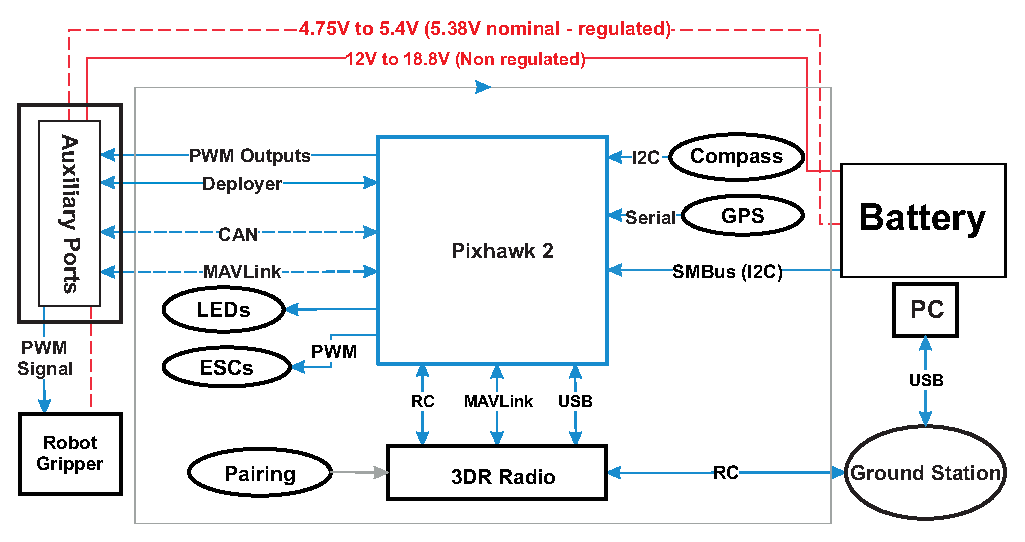
\includegraphics[width=\columnwidth]{arquiteturaIHW.eps}
	\caption{System Hardware Architecture.}
	\label{fig:hardArch}
\end{figure}

In the software architecture, the mission planner (cf. Definition~\ref{def:planejadorMissao}) reads the warehouse inputs and client order and generates the production mission, which contains the list of mission commands needed for producing the required client order. Figure~\ref{fig:sysArch} shows the mission planning framework software components.


In order to control the UAV from a Android application, we have used the dronekit API that translates MAVLink commands to a Java function. The application talks to the UAV using a radio module connected via USB. We have created a bunch of functions in the control program for the most common UAV actions. The movement functions (cf. Definition~\ref{def:movFunc}) are described in Table~\ref{table:movfunc}.
%
%\begin{itemize}
%\item \texttt{TakeOff}: takeoff command of the UAV;
%\item \texttt{GoTo}: command to move the  UAV to a certain location;
%\item \texttt{TakePackage}: command to collect an input/product through a robot gripper;
%\item \texttt{LeavePackage}: command to leave an input or product from a robot gripper;
%\item \texttt{Wait}: command to make a UAV to hover (wait);
%\item \texttt{Land}: command to make a UAV to land.
%\end{itemize}

\begin{table}[]
\scriptsize
\centering
\begin{tabular}{|l|l|}
\hline
\multicolumn{1}{|c|}{\textbf{Command}} & \multicolumn{1}{c|}{\textbf{Description}}           \\ \hline
\texttt{TakeOff}                     & takes off the UAV                                   \\ \hline
\texttt{GoTo}                        & moves the UAV to a certain location                 \\ \hline
\texttt{TakePackage}                 & takes an input/product (gripper) \\ \hline
\texttt{LeavePackage}                & leaves an input/product (gripper)   \\ \hline
\texttt{Wait}                        & makes the UAV to hover (wait)                       \\ \hline
\texttt{Land}                        & lands the UAV                                       \\ \hline
\end{tabular}
\caption{Description of movement functions}
\label{table:movfunc}
\end{table}


\begin{figure}[H]
	\centering
	\includegraphics[width=\columnwidth]{sysArch.eps}
	\caption{System's Architecture.\label{fig:sysArch}}
\end{figure}


%\subsection{Mission Planning}
%\label{mission}


%%%%%%%%%%%%%%%
\section{Methodology}
\label{sec:method}
%%%%%%%%%%%%%%%

%\commentib{Modifique o t\'itulo (expanda). Metodologia de qu\^e?? Tente fazer algo parecido com o do trabalho.}

%In this section, we evaluate the algorithm mission cost and describe a case study to a UAV and contents about mission planning.

%%%%%%%%%%%%%%%%%%%%%%%%%%%%%%%%%%%%%
\subsection{Case Study: UAV Intralogistics Mission}
\label{sec:ec}
%%%%%%%%%%%%%%%%%%%%%%%%%%%%%%%%%%%%%

In order to model the mission planning problem as an optimization problem, the case study shown in Figure~\ref{fig:useCase} is used.
%
\begin{figure}[ht]
	\centering
	\includegraphics[width=0.85\columnwidth]{useCase.eps}
	\caption{Case Study Representation.\label{fig:useCase}}
\end{figure}
	
Figure~\ref{fig:useCase} shows that there are three types of inputs in the warehouse (\textit{i.e.}, A, B, and C) and two production lines that produce two different products (\textit{i.e.}, X and Y). Each production line produces only one type of product and has a characteristic production time (cf. Definition~\ref{def:tempoProducao}). Figure~\ref{fig:useCase} shows that to produce a product of type X, two inputs of type A and one input of type C are required, and to produce a product of type Y, two inputs of type B and one input of type C are required. The production time of a X product is $4 p.u.$ and the time of production of product Y is $6 p.u.$. A production unit ($1 p.u.$) is considered to be a \texttt{GoTo} command performed by the UAV.

The task to be performed is the production of the client order (cf. Definition~\ref{def:pedido}), where a given UAV collects supplies from the warehouse, takes that to the production line, and once the production of a certain product is finished, the UAV delivers it to the client.

\subsection{UAV Controller App}
\label{subsec:app}

We developed an Android application to connect to the UAV via usb (radio signal module) or udp (simulated uav) in order to create a client order and make the UAV executes it autonomously and the user can visualize and supervise the operation.

\begin{figure}[H]
\centering
\begin{minipage}{.25\textwidth}
  \centering
  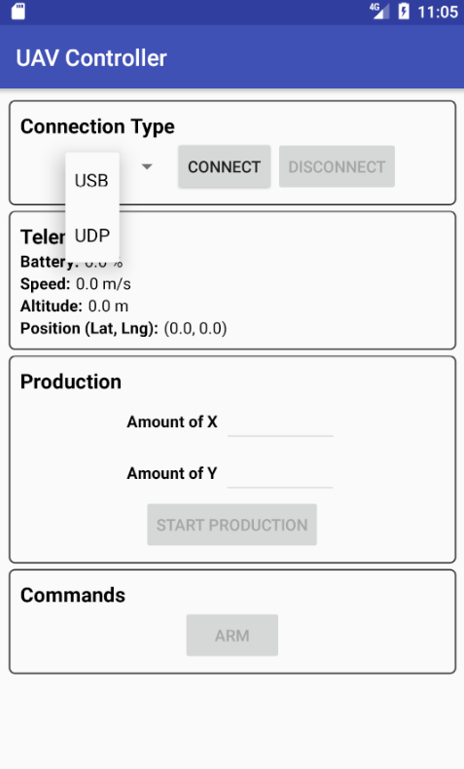
\includegraphics[width=.7\linewidth]{appMain}
  \captionof{figure}{Main Screen.}
  \label{fig:appMain}
\end{minipage}%
\begin{minipage}{.25\textwidth}
  \centering
  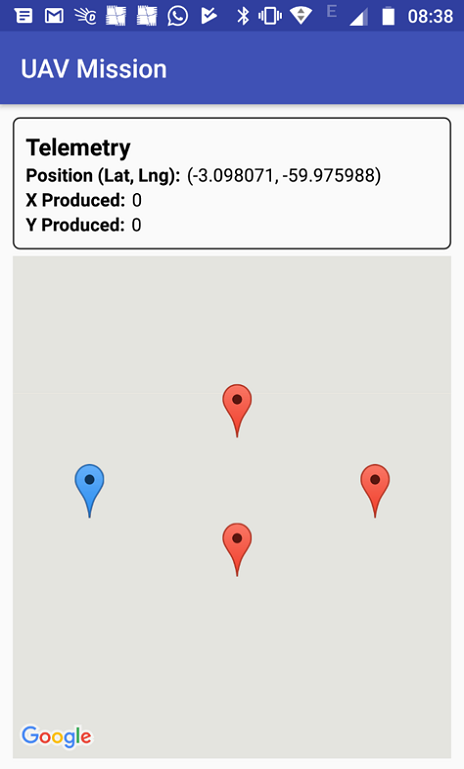
\includegraphics[width=.7\linewidth]{appSec}
  \captionof{figure}{Secondary Screen.}
  \label{fig:appSec}
\end{minipage}
\end{figure}

Internally in the app, it's implemented the mission planner and the controller module to send commands to the UAV via radio using the MAVLink protocol in the dronekit API.

%%%%%%%%%%%%%%%%%%%%%%%%%%%%%%%%%%%%%
\section{Experimental Evaluation}
\label{sec:results}
%%%%%%%%%%%%%%%%%%%%%%%%%%%%%%%%%%%%%
In this section we present the experimental results of the Android application to control a UAV as described in Section~\ref{sec:ec}.

The Table~\ref{table:tests} shows the experiments tested in a real UAV and a virtual UAV, in order to compare the results in both environments. As we present, when the virtual UAV is used, the mission gets a smaller flight time than in the real UAV. That is because the radio communication used in the real drone is affected by noises in the environment.
\begin{table}[H]
\centering
\begin{tabular}{@{}ccc@{}}
\cmidrule(l){2-3}
                                        & \cellcolor[HTML]{FF7774}\textbf{Real UAV} & \cellcolor[HTML]{5FCE89}\textbf{Virtual UAV} \\ \cmidrule(l){2-3} 
\cellcolor[HTML]{C0C0C0}\textbf{Tests} & \textit{\textbf{Flight Time (s)}}            & \textit{\textbf{Flight Time (s)}}            \\
\cellcolor[HTML]{C0C0C0}1               & 441.72                                       & 430.830                                       \\
\cellcolor[HTML]{C0C0C0}2               & 440.18                                       & 436.885                                       \\
\cellcolor[HTML]{C0C0C0}3               & 447.51                                       & 441.681                                       \\
\cellcolor[HTML]{C0C0C0}4               & 438.19                                       & 441.277                                       \\
\cellcolor[HTML]{C0C0C0}5               & 445.85                                       & 451.865                                       \\ \bottomrule
\end{tabular}
\caption{Mission Flight Time Tested in Real and Virtual UAV.\label{table:tests}}
\end{table}


\section{Conclusion}
\label{sec:conclusao}
%---------------------------------

We have presented an evaluation methodology for UAV mission planner in an industrial production scenario, as described in Section~\ref{sec:method}. We have developed an Android application to supervise production status and allow real-time monitoring for line managers/leaders.
 
In addition, we have developed a framework for mission planning, command and control for intralogistics mission using a commercial UAV. We used an UAV to solve intralogistics problems using the dronekit API to control and command adopting a high-level programming language.

Future work includes the use of computational vision for the recognition of inputs, and improvements of the optimization problem modeling for better results in cost evaluation. Supplementary, we will make experiments in a cooperative work environment where the number of UAVs is greater than two. In order to improve our results, we will develop more planner strategies such as an algorithm that produces different types of products simultaneously. Moreover, we will evaluate the communication between the drone and the application using different frameworks/protocols, in order to improve the supervision step.

\bibliographystyle{IEEEtran}
\bibliography{IEEEabrv,exemplo}

\end{document}


